\chapter{格子Boltzmann方法基本原理}\label{chp:LBM}

\section{LBM基本模型}
格子Boltzmann方法(LBM)是一种求解Navier-Stokes方程的方法。在历史上由格子气自动机发展而来的,
但其核心方程\---格子Boltzmann方程(LBE)也可以由连续Boltzmann方程推导出来。
它可以看做是连续Boltzmann方程在速度空间和几何位置空间的离散化形式。LBE描述的是离散几何空间中
粒子速度分布函数的演化规则:
%% 的速度分布函数的演化过程:
\begin{equation}
  f_i(\bm{x}+\bm{c}_i\delta t,t+\delta t) - f_i(\bm{x},t) = \Omega_i\left(f(\bm x, t)\right)
  \label{lbe}
\end{equation}
其中$f_i(\bm x,t)$是速度分布函数,表示在时刻$t$,占据空间位置$\bm{x}$处的粒子具有离散速度$\bm{c}_i$的
概率,$\delta t$是相邻演化步时间间隔。等式右边$\Omega_i$是碰撞算子,表示演化过程相邻粒子之间的
相互作用对速度分布函数的影响。
格点上的宏观量如密度$\rho$、速度$\bm u$由速度分布函数求得:
\begin{equation}
  \rho = \sum_i f_i, \quad 、\rho\bm u = \sum_i f_i \bm c_i
  \label{macro}
\end{equation}

LBE方程在计算上可以分为两个步骤,
即碰撞步
\begin{equation}
  f'_i(\bm x, t) = f_i(\bm{x},t) + \Omega_i\left(f(\bm x, t)\right)
  \label{lbe-collision}
\end{equation}
和迁移步
\begin{equation}
 f_i(\bm{x}+\bm{c}_i\delta t,t+\delta t) = f_i(\bm{x},t)
  \label{lbe-stream}
\end{equation}
粒子之间的碰撞要求满足质量守恒,动量守恒,即要求碰撞算子满足:
\begin{equation}
 \sum_i \Omega_i(f) = 0, \quad \sum_i \Omega_i(f)\bm c_i = 0。
  \label{conservation}
\end{equation}

最简单碰撞算子$\Omega_i$模型是由Qian等人提出的DnQb LBGK模型\ucite{qian1992lattice},
相对于后来提出的多松弛时间模型,它也被称作单松弛时间模型。在LBGK模型中,$\Omega_i$的形式为:
\begin{equation}
 \Omega_i(f) = -\frac{1}{\tau}\left( f_i  - f_i^{eq}\right)
  \label{lbgk}
\end{equation}
其中$\tau$为无量纲松弛时间,与流体动力学粘性关联
\begin{equation}
  \nu = c_s^2(\tau-\frac{1}{2})\delta t
  \label{nu_tau}
  \end{equation}
$f_i^{eq}$为平衡态分布函数,由格点的宏观量决定:
\begin{equation}
  f_i^{eq} = \omega_i \rho 
  \left[ 1 
    + \frac{\bm c_i \cdot \bm u}{c_s^2}
    + \frac{(\bm c_i \cdot \bm u)^2}{2c_s^4}
    - \frac{u^2}{2c_s^2}
    \right]
  \label{feq}
\end{equation}
其中$\omega_i$为权系数, $c_s=\sqrt{RT}$与声速有关的常数。本文使用的主要的三维格子为D3Q19模型,
其离散速度为:
\begin{displaymath}
\small
  \bm c =  \left[\begin{array}{*{19}{r}}
 0 & 1 & -1 & 0 & 0 & 0 & 0 & 0 & 0 & 0 & 0 & -1 & 1 & -1 & 1 & -1 & 1 & -1 & 1 \\
 0 & 0 & 0 & 1 & -1 & 0 & 0 & 1 & -1 & -1 & 1 & 0 & 0 & 0 & 0 & 1 & -1 & -1 & 1 \\
 0 & 0 & 0 & 0 & 0 & 1 & -1 & 1 & -1 & 1 & -1 & -1 & 1 & 1 & -1 & 0 & 0 & 0 & 0
\end{array}\right] c
\end{displaymath}
其中$c$为格子速度,定义为格子长度与时间步长之比,即$c=\frac{\delta x}{\delta t}$
。$c_s$和$\omega_i$分别为:
\begin{displaymath}
c_s = \frac{c}{\sqrt{3}}, \quad
\omega_i =\left\{ \begin{array}{ll}
1/3 & c_i^2=0 \\
1/18 & c_i^2=c^2 \\
1/36 & c_i^2=2c^2 
\end{array}\right.
\end{displaymath}
图\ref{fig:d3q19}为D3Q19格子模型离散速度示意图。

%  计算区域被离散为规则排布的空间格点,粒子就是在这些离散格点上碰撞并按照离散速度方向迁移到相邻格点。
%按Qian等人提出的DnQb模型,常用的二维格子模型有D2Q9,三维模型有D3Q15、D3Q19等,这里详细描述本文用到的主要
%模型\--- D3Q19模型。
\begin{figure}[htpb]
  \centering
  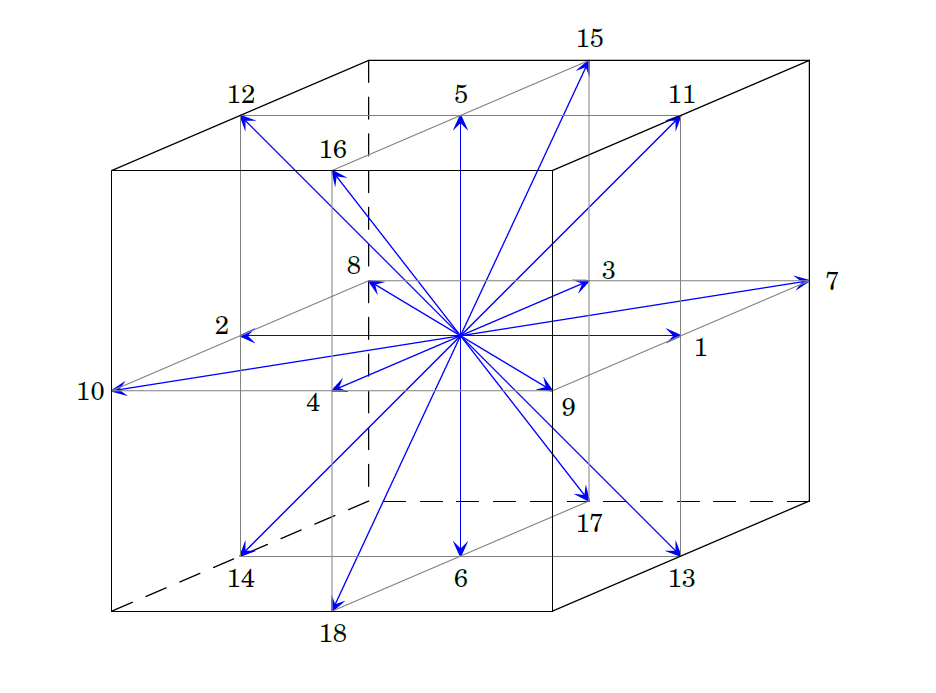
\includegraphics[width=0.5\textwidth]{img/d3q19}
  \caption{D3Q19模型离散速度}
  \label{fig:d3q19}
\end{figure}





%
%$\Omega_i$通常只由当前格点自己的各个速度方向的速度分布函数$f_i(\bm x, t)$决定,因此LBE是一种显式格式。
%在碰撞步,各个个格点的速度分布函数更新操作可以独立进行,并且只涉及到读取本身的信息,
%因此非常适合于细粒度的并行。

%传统的CFD方法如有限差分法、有限体积法、有限元法都是采用数值格式离散Navier-Stokes偏微分方程,
%得到一组线性方程组,然后采用数值线性代数的方法求解这组方程组从而得到流场在离散单元上的离散解。
%这些方法可以看做是“自顶向下”的方法,即已知描述流体运动规律的宏观控制方程,然后标准的偏微分
%方程求解方法来求解它们。而LBM与这些方法不同,它更类似于分子动力学方法(MD),即从微观上描述
%一群粒子的运动过程。在给定初始状态和演化规则的情况下,可以知道粒子在任一时刻的分布状态。
%但与MD描述每个真实分子的运动状态不同,LBM采用的是统计力学的方法,描述

\section{多松弛时间模型}
在LBGK模型中,各个方向的速度分布函数的松弛时间都是$\tau$,所以也被称作单松弛时间模型。
另一种常用的碰撞算子模型是多松弛时间模型(MRT), Lallemannd 和 Luo曾对这一模型做过
细致的理论分析,证明该模型比LBGK模型在参数选择自由度和数值稳定性方面具有更大优势,
并且物理原理更清晰。值得指出在LBGK在模拟多孔介质流动时,会得到绝对渗透率与流体
粘性相关联的非物理结果,而MRT模型则可以大大改善这一问题,Pan等人对这一问题做了详细算例验证
和分析\ucite{pan2006evaluation}。
MRT模型与LBGK模型不同之处在于它的碰撞过程是在矩空间中完成的。
碰撞前速度分布函数被一个正交变换矩阵$\bm M$映射到矩空间:
\begin{equation}
  m = \bm M \cdot \bm f
  \label{M_to_f}
\end{equation}
其中$m$为矩向量,对于D3Q19模型,$\bm M$为
  \renewcommand{\baselinestretch}{1.25}
\begin{displaymath}
\footnotesize
\bm M = \left(
\begin{array}{*{19}{@{\hspace{5pt}}r}}
 1 & 1 & 1 & 1 & 1 & 1 & 1 & 1 & 1 & 1 & 1 & 1 & 1 & 1 & 1 & 1 & 1 & 1 & 1 \\
 -30 & -11 & -11 & -11 & -11 & -11 & -11 & 8 & 8 & 8 & 8 & 8 & 8 & 8 & 8 & 8 & 8 & 8 & 8 \\
 12 & -4 & -4 & -4 & -4 & -4 & -4 & 1 & 1 & 1 & 1 & 1 & 1 & 1 & 1 & 1 & 1 & 1 & 1 \\
 0 & 1 & -1 & 0 & 0 & 0 & 0 & 0 & 0 & 0 & 0 & -1 & 1 & -1 & 1 & -1 & 1 & -1 & 1 \\
 0 & -4 & 4 & 0 & 0 & 0 & 0 & 0 & 0 & 0 & 0 & -1 & 1 & -1 & 1 & -1 & 1 & -1 & 1 \\
 0 & 0 & 0 & 1 & -1 & 0 & 0 & 1 & -1 & -1 & 1 & 0 & 0 & 0 & 0 & 1 & -1 & -1 & 1 \\
 0 & 0 & 0 & -4 & 4 & 0 & 0 & 1 & -1 & -1 & 1 & 0 & 0 & 0 & 0 & 1 & -1 & -1 & 1 \\
 0 & 0 & 0 & 0 & 0 & 1 & -1 & 1 & -1 & 1 & -1 & -1 & 1 & 1 & -1 & 0 & 0 & 0 & 0 \\
 0 & 0 & 0 & 0 & 0 & -4 & 4 & 1 & -1 & 1 & -1 & -1 & 1 & 1 & -1 & 0 & 0 & 0 & 0 \\
 0 & 2 & 2 & -1 & -1 & -1 & -1 & -2 & -2 & -2 & -2 & 1 & 1 & 1 & 1 & 1 & 1 & 1 & 1 \\
 0 & -4 & -4 & 2 & 2 & 2 & 2 & -2 & -2 & -2 & -2 & 1 & 1 & 1 & 1 & 1 & 1 & 1 & 1 \\
 0 & 0 & 0 & 1 & 1 & -1 & -1 & 0 & 0 & 0 & 0 & -1 & -1 & -1 & -1 & 1 & 1 & 1 & 1 \\
 0 & 0 & 0 & -2 & -2 & 2 & 2 & 0 & 0 & 0 & 0 & -1 & -1 & -1 & -1 & 1 & 1 & 1 & 1 \\
 0 & 0 & 0 & 0 & 0 & 0 & 0 & 0 & 0 & 0 & 0 & 0 & 0 & 0 & 0 & -1 & -1 & 1 & 1 \\
 0 & 0 & 0 & 0 & 0 & 0 & 0 & 1 & 1 & -1 & -1 & 0 & 0 & 0 & 0 & 0 & 0 & 0 & 0 \\
 0 & 0 & 0 & 0 & 0 & 0 & 0 & 0 & 0 & 0 & 0 & 1 & 1 & -1 & -1 & 0 & 0 & 0 & 0 \\
 0 & 0 & 0 & 0 & 0 & 0 & 0 & 0 & 0 & 0 & 0 & 1 & -1 & 1 & -1 & -1 & 1 & -1 & 1 \\
 0 & 0 & 0 & 0 & 0 & 0 & 0 & 1 & -1 & -1 & 1 & 0 & 0 & 0 & 0 & -1 & 1 & 1 & -1 \\
 0 & 0 & 0 & 0 & 0 & 0 & 0 & -1 & 1 & -1 & 1 & -1 & 1 & 1 & -1 & 0 & 0 & 0 & 0
\end{array}
\right)
\end{displaymath}
 \renewcommand{\baselinestretch}{1.5}
相应的矩向量为
\begin{displaymath}
 m=(\rho, e, \epsilon, j_x, q_x, j_y, q_y, j_z, q_z, 
3p_{xx}, 3\pi_{xx},p_{ww},\pi_{ww},p_{xy}, p_{yz}, p_{zx},m_x, m_y, m_z)
\end{displaymath}
其中各分量的意义及其对应的平衡态形式见参考文献\cite{pan2006evaluation},此处不再详细给出。
%其中$e$是能量,$\epsilon$是能量的平方,$\bm j=(j_x, j_y, j_z)$是动量,$\bm q=(q_x, q_y, q_z)$
%是热通量,$p_{xx},p_{ww}, p_{xy}, p_{yz}, p_{zx}$是与应力张量直接相关的矩,$\pi_{xx}, \pi_{ww}$
%是四阶矩,$m=(m_x, m_y, m_z)$是与速度有关的三阶矩。其中的$\rho$和$\bm j$是守恒矩。矩向量的平衡态
%$\bm m^{eq}$为
% m=(\rho, e, \epsilon, j_x, q_x, j_y, q_y, j_z, q_z, 
%3p_{xx}, 3\pi_{xx},p_{ww},\pi_{ww},p_{xy}, p_{yz}, p_{zx},m_x, m_y, m_z)
%\end{displaymath}


MRT模型中碰撞时先将$\bm f$转换到矩空间得到矩向量$\bm m$,
然后在矩空间完成碰撞,最后把碰撞更新后的$m$转换回速度分布函数$\bm f$,整个过程可以表示为
\begin{equation}
\Omega_i = \bm M^{-1} \bm S(\bm m - \bm m^{eq})
\end{equation}
其中$\bm S$为对角矩阵,其对角线上的各个元素为矩向量各分量的无量纲松弛时间, 其形式为
\begin{displaymath}
\bm S = diag(0,s_1,s_2,0,s_4, 0, s_4, 0, s_4, s_9, s_10, s_9, s_{10}, s_{13}, s_{13}, s_{13}, s_{16}, s_{16}, s_{16})
\end{displaymath}
通常取$s_9=s_{13}=s_\nu$, $s_\nu$与流体动力学粘性相关
\begin{equation}
\nu = c_s^2(\frac{1}{s_\nu}-\frac{1}{2})\delta t
\end{equation}
其它松弛时间可自由调节以获得更高的稳定性\ucite{d2002multiple}。


%%%%%%%%%%%%%%%%%%%%%%%%%%%%%%%%%%%%%%%%%%%%%%%%%%%%%%%%%%%%%%%%%%%%%%%%%%%%%%%%%%%%
\section{边界处理}
在迁移过程中,处于流场边界上的格点需要特殊处理,因为边界以外没有粒子迁移到这些格点,
LBM的边界处理的目标就是根据给定的宏观边界条件构造出这些未知的粒子分布函数。在这一节中
笔者主要讨论本文用到的三种边界处理格式,分别为周期性边界条件、反弹格式及郭照立提出的
非平衡外推格式\ucite{guo2002extrapolation}。

\begin{myDescription}
\item[周期性边界条件]
某些问题流场本身就有空间周期性, 这时可以只求解一个周期单元。这种边界处理在LB里面处理
非常容易,当前时间步从一侧流入流场的粒子就是上一时刻从另一侧流入流场的粒子。

\item[反弹格式]
反弹格式是来处理无滑移速度壁面最简单的,并且物理背景清晰。其基本想法是认为
靠经壁面的格点上的粒子在当前时间步流动到壁面并与壁面反弹后由其反方向弹回,在下一时间步
正好又回到这个格点。这种格式自动满足质量守恒和动量守恒。需要注意的是,标准
如果反弹格式中靠近壁面执行反弹的格点本身不执行碰撞更新操作,则称该格式为标准反弹格式,否则
为修正反弹格式,前者仅具有一阶精度,而后者具有二阶精度。另一种具有二阶精度的反弹格式为
Half-Way反弹格式,这种格式假设壁面正好位于格点连线之间。

\item[非平衡外推格式]
非平衡外推的基本思想是将边界格点上未知的分布函数分为平衡态和非平衡态部分,其中非平衡
部分,由临近的流场内部格点的非平衡部分一阶外推得到,而平衡态部分则根据给定的边界宏观量
来构造,构造过程缺少的宏观量也由临近的流场内部格点上的相应宏观量外推得到。这种格式整体
精度是二阶的\ucite{guoredbook}。
\end{myDescription}

%%%%%%%%%%%%%%%%%%%%%%%%%%%%%%%%%%%%%%%%%%%%%%%%%%%%%%%%%%%%%%%%%%%%%%%%%%%%%%%%%%%%
\section{多相/多组分LBE模型}\label{sec:lbm_multiphase}
宏观的相间相互作用本质上是组分中微观分子间的相互作用,因此如果能准确描述这种
分子间相互作用,则宏观多相/多组分复杂的流动现象会自然体现出来。LBM的微观本质和介观特点
决定了LBM也可以通过构造粒子间相互作用模型来模拟多相/多组分流动。目前在LBM中,描述粒子
间相互作用的方式有颜色模型、伪势模型、自由能模型和动力学模型。其中伪势模型又称Shan-Chen
模型,是由Shan和Chen于1993年提出的\ucite{sc93}。该模型假设流体粒子之间存在一种非局部的
相互作用,并通过引入一种势函数来描述这种相互作用,作用力的大小就是势函数的梯度。该模型
提出后,针对其存在的问题,又有多种改进模型被提出。本文所采用的多相多组分模型
\ucite{porter2012multicomponent}就是针对对Shan-Chen模型的一种改进。该模型主要解决了
Shan-Chen模型中平衡态密度和粘度相关的问题,并且能过模拟大粘度比的组分。下面将以该模型
为背景简要介绍运用LBM模拟多组分/多相问题的要点。

\subsection{组分间相互作用}
在原始的Shan-Chen模型中,组分间的相互作用力通过一个势函数来描述,
并且这个相互作用力对碰撞过程的影响通过校正有效平衡态速度来体现\ucite{sc93}。相互作用力的表达式为
\begin{equation}
\bm F_k(\bm x) = -\psi_k(\bm x)\sum_{\bar k}g_{k\bar k}\sum_i\psi_{\bar k}(\bm x+\bm c_i\delta t)\bm c_i
\label{sc_force}
\end{equation}
其中$\psi_k$是势函数,对于多组分模型通常就取为组分的密度即,$\psi_k = \rho_k$。$g_{k{\bar k}}$是反映
组分粒子间相互作用的系数。
在本文使用的这个模型中,每个组分所受到的合外力显式(explict force )的加到了其格子Boltzmann方程中\ucite{porter2012multicomponent},后文中称这种模型为EF模型。每个组分的LBE为
\begin{equation}
f_i^k(\bm x + \bm c_i\delta t) - f_i^k(\bm x, t)=\Omega_i^k(f(\bm x, t))+\frac{\Delta t}{2}
\left[ f_i^{F,k}(\bm x+\delta t, t+\delta t)+ f_i^{F,k}(\bm x, t)\right]
\label{ef_lbe}
\end{equation}
其中的$f_i^{F,k}$是粒子所受合外力引起的速度分布函数的改变,碰撞算子$\Omega_i$与单组分LBE形式相同。
$f_i^{F,k}$定义为
\begin{equation}
f_i^{F,k}=\frac{\bm F_k \cdot(\bm c_i - \bm u_{eq})}{\rho_k c_s^2}f_i^{eq,k}
\end{equation}
其中$\bm F_k$为组分$k$的粒子所受外力,包括组分间作用力。$\bm u^{eq}$是有效速度,定义为
\begin{equation}
\bm u^{eq} =  \sum_k\frac{\rho_k \bm u_k}{\tau_k}/\sum_k\frac{\rho_k}{\tau_k}
\end{equation}

方程\eqref{ef_lbe}右端包含新时间步的变量,所以是显式形式,通过做代换
$\bar f_i^k=f_i^k -\frac{\delta t}{2}f_i^{F,k}$,该方程可变为显式形式
\begin{equation}
\bar f_i^k(\bm x + \bm c_i\delta t) - \bar f_i^k(\bm x, t) 
=\frac{1}{\tau_k}\left[f_i^{eq,k}(\bm x, t) - \bar f_i^k(\bm x, t) - \frac{\delta t}{2}f_i^{F,k}\right]
+\delta t f_i^{F,k}
\end{equation}
每个组分的宏观量定义为
\begin{equation}
\rho_k = \sum_i\bar f_i^k, \quad \rho_k \bm u_k = \sum_i \bar f_i^k \bm c_i + \frac{\delta t}{2}\bm F_k
\end{equation}
混合流体的真实速度为
\begin{equation}
\bm u =\frac{\sum\nolimits_k\rho_k\bm u_k}{\sum\nolimits_k\rho_k}
\end{equation}
流体状态方程为
\begin{equation}
  p=c_s^2 \sum_k\rho_k + \frac{c_0}{2}\sum_{k\bar k}g_{k\bar k}\psi_k\psi_{\bar k}
  \label{EOS}
\end{equation}

值得指出的是在原文献\ucite{porter2012multicomponent}中,为能模拟大粘度比组分,
式\eqref{sc_force}表达为
\begin{equation}
\bm F_k(\bm x) = -c_0\psi_k(\bm x)\sum_{\bar k}g_{k\bar k}\nabla \psi_{\bar k}(\bm x)
\label{sc_force_m}
\end{equation}
式中$c_0$是个常速,对于D3Q19格子模型,$c_0 =6$,式中的梯度算子
用具有较好各向同性的的高阶差分算法替代。但考虑到GPU上对显存访问的特殊要求(见\ref{sec:cuda_principle}节中的
解释),我们在后文中实现的多组分GPU程序使用的都是一阶中心差分格式。

\subsection{流固界面相互作用}
流固边界处的流体格点的某些方向上的相邻格点可能是固体格点,为反映固体边界对各组分的作用,
可以将固体格点等效为另一种假想的组分,其密度为常数$\rho_s$,它与流体组分间的相互作用系数
用$g_{ks}$替代,$g_{ks}$大小反应组分$k$对该固体表面的润湿性,通过调整不同组分的$g_{ks}$
控制相界面接触角的大小\ucite{pan2004lattice}。

%在多组分流中,每个组分有自己的分布函数,并且它们的演化过程都满足格子Boltzmann方程
%\begin{equation}
%f_i^k(\bm x + \bm c_i\delta t) - f_i^k(\bm x, t)=\Omega_i^k(f(\bm x, t))
%\end{equation}
%其中$k$表示组分,由于本文只涉及到两组分,所以$k$取值为$1$或$2$。当然也很容易扩展成更多
%组分。如果采用单松弛碰撞算子模型则有
%\begin{equation}
%\Omega_i^k = \frac{f_i^{eq,k}(\bm x, t) - f_i^k(\bm x, t)}{\tau_k}
%\label{srt_multi}
%\end{equation}
%其中$\tau_k$表示组分$k$的无量纲松弛时间,同单组份的LBM一样分别于两种组分的动力学粘性相关,
%式中中各组分$f_i^{eq,k}$平衡态定义如下
%\begin{equation}
%  f_i^{eq,k} = \omega_i \rho_k 
%  \left[ 1 
%    + \frac{\bm c_i \cdot \bm u_k^{eq}}{c_s^2}
%    + \frac{(\bm c_i \cdot \bm u_k^{eq})^2}{2c_s^4}
%    - \frac{u^{eq}\cdot u^{eq}}{2c_s^2}
%    \right]
%  \label{feq_multi}
%\end{equation}
%每个组分的宏观量$\rho_k$、$\bm u_k$依然按各自的分布函数统计出来,即
%\begin{equation}
% \rho_k = \sum_i f_i, \quad \rho_k \bm u_k =  \bm c_i f_i
%\end{equation}
%式\eqref{feq_multi}中的$\bm u^{eq}$是根据组分间相互作用力校正过了的有效速度
%\begin{equation}
% \rho_k \bm u
%\end{equation}

%%%%%%%%%%%%%%%%%%%%%%%%%%%%%%%%%%%%%%%%%%%%%%%%%%%%%%%%%%%%%%%%%%%%%%%%%%%%%%%%%%%%
\section{小节}
本章介绍了LBM基本原理。在第一节中介绍了常用的D2Q9和D3Q19格子模型,以及单松弛时间(LBGK)模型,
第二节介绍了后文将要使用的多松弛时间(MRT)模型,第三节介绍了常用的LB边界处理方法。
第四节详细介绍了本文所使用多相LB模型。







